\openingarticle
\def\ppages{\pagerange{heekeren:firstpage}{heekeren:lastpage}}
\def\shorttitle{A Method and an Object}
\def\maintitle{A Method and an Object: An Art Historical Approach Applied to the ‘Memento-Mori’ Mosaic from Pompeii, Italy}
\def\shortauthor{Vivian S. van Heekeren}
\def\authormail{v.s.van.heekeren@umail.leidenuniv.nl}
\def\affiliation{Leiden University}
\def\thanknote{\footnote{Vivian S. van Heekeren is an undergraduate student at the Faculty of Archaeology at University Leiden (Netherlands). She is currently working towards her bachelor’s degree in archaeology. Her thesis is focussed on metabolic bone disease in post-medieval Britain. She is interested in human osteology, funerary archaeology, paleopathology and the interaction in ancient societies between the living and the dead (rite de passage). She is also broadly interested in museum studies, Roman archaeology and ancient Near Eastern archaeology. 	In the future, she would like to undertake postgraduate studies and proceed a career in academic research.}}
%--------------------------------------------------------------
\mychapter{A Method and an Object:\\ An Art Historical Approach Applied to the ‘Memento-Mori’ Mosaic from Pompeii, Italy}
\begin{center}
	{\Large\scshape\shortauthor \thanknote}\\[1em]
	\email \\
	\affiliation
\end{center}
\vspace{3em}
\midarticle
%--------------------------------------------------------------
\label{heekeren:firstpage}

	%----------------------------------------------------------------------------------------
	\begin{myabstract}Roman\marginnote{Abstract\\ (in Italian see below)} objects and art has been a source of fruitful discussion between scholars, and has led to the development of subsequent theories. Traditional research has been influenced for instance by Winckelmann and the Kopienkritik. These theories have been useful in understanding Roman art, but lack an objective approach. In 1939, Erwin Panofsky published his book Studies in Iconology. He introduced a three-levelled approach for structured iconographical analyses of Renaissance art. This article investigates the application of Panofsky’s three-levelled approach to a Roman Memento-Mori mosaic to see whether it is useful for understanding archaeological objects. The aim is to develop a multidisciplinary, contextualised visual analysis of the object with a crossover of techniques between archaeology and art history, in order to assess its suitability for the interpretation of past material culture		
		
	\keywords[Keywords]{Erwin Panofsky, Pompeii, Mosaic, Memento Mori, Roman art, Iconography, Iconology.}
	\end{myabstract}
	

\lettrine[nindent=0em,lines=3]{A}{rt} has played an important role in the development of archaeology as a discipline, because many items of material culture have been preserved and recovered due to their aesthetic qualities. The associations with the term art are various and depend on cultural backgrounds, different ages, and critical attitudes \parencite [309-310] {LaRocca_2010}. Objects don’t have a single meaning fixed in a moment of time. The interpretation of the viewer would have been influenced by the intellectual, social, and political background, especially in the absence of explanatory texts as is now practiced in most museums \parencite [49] {Rose_2010}. By exploring archaeological objects through iconographical analysis, it is possible to obtain new insights in the worldviews of ancient societies. In 1939, Erwin Panofsky published his book Studies in Iconology. Even though this book was written for Renaissance period art, its approach remains applicable across periods, an approach focused on the intrinsic meaning of art. In this study, Panofsky defined a distinction between meaning and form by a three-levelled approach, applying it to Renaissance period art. 

	The meaning of objects are subject to reinterpretation by new generations of scholars, as argued by \textcite [71]{Rose_2010}, to be discussed in this paper. The paper focuses on the utility of Panofsky’s approach for interpreting Roman objects. Is this approach helpful for understanding the iconography of a Roman object? To find the answer, this method will be applied to the ‘Memento Mori’ mosaic from Pompeii, Italy. The case study that has been chosen is a complicated piece with many different elements. Even though Panofsky’s approach is an older method, it could still prove to be relevant for iconographical analysis. In this article I briefly introduce the relationship between art and archaeology, followed by an explanation of how Panofsky’s method works and how it could be applied. I then present the analysis of the case study, described in several sections, each one discussing a different part of the ‘Memento Mori’ (reminders of death) mosaic. Finally, I conclude with a discussion on the applicability of the approach to the interpretation of art objects. 
	
%\section{History of Visual Culture in Art and Archaeology}
Before\marginnote{History of Visual Culture in Art and Archaeology} Panofsky’s method can be applied to the case study used in this paper, it is important to mention other influential approaches to visual culture in archaeology. This is done in order to demonstrate the difference Panofsky’s approach. Generally, scholars refer to Winckelmann as the ‘father’ of art history. He published his book Geschichte der Kunst des Alterthums (‘History of Art of Antiquity’) in 1764, containing a chronical schema for plotting the development of ancient art, and identifying four main stages within this schema \parencite[68--69] {BeardHenderson_2001}. These four periods are the ‘Older Style’, ‘High Style’, ‘Beautiful Style’, and the ‘Style of the Imitators’. According to \textcite {BeardHenderson_2001}  it is possible to trace back all art history to Winckelmann’s basic schema.

	The Kopienkritik theory, practiced since the nineteenth century, labelled Roman art as “free” copies of lost Greek originals. German scholars, led by Heinrich Brunn, tried to reconstruct the lost Greek originals by comparing photographs with the existing sculptural copies. The Kopienkritik theory is mainly based on statues, but might have also influenced the interpretation of other art forms within the Roman context \parencites{Perry_2005}[4--6]{Gazda_2002}. This approach was followed by the Idealplastik theory, introduced by German scholars in the 1970’s. Thereafter, the three forms - interpretation, imitation, and emulation- made their appearance. These were followed by postmodern reformulations from the 1980’s onwards \parencite[7--9]{Gazda_2002} . 
	There is a heated debate amongst scholars around the originality of the Roman artistic culture \parencite {LaRocca_2010}. Roman art seems to be derived from the supreme Greek counterpart. It is also argued that Roman art lacks any coherent line of evolution, and that it has strongly been influenced by geographic inflection, so much so that it does not consist of an autonomous artistic language \parencite [344--345] {LaRocca_2010}. 
	According to \textcite{Perry_2005}, there are three aesthetic concepts that apply to and influence Roman art. The first concept is decorum, which required that works of art be bespoke to their specific contexts. This could be in an architectural, social, or thematic way. Decorum is contrary to the Kopienkritik theory, as the resulting pieces of art comprise a much more varied corpus than exact copies could provide. This then suggests that the Roman understanding of artistic imitation is different. The next concept is the aesthetic of eclecticism, which allowed an artist to introduce a new innovative idea to fit in the tradition of decorum. The last concept, phantasia, represents the artistic visualisation. The representations of gods and heroes were not produced by ‘copying’ another artwork, but by the reproduction of a vision that the artist had in mind \parencite {Perry_2005}. Notably, there is much debate regarding these theories with an ongoing search for alternative theories \parencite [16]{Gazda_2002}. 
	
%	\section{Iconology by Panofsky}
In\marginnote{Iconology by Panofsky} this article I explore the applicability of Panofsky’s approach to Roman objects. This three-levelled method by \textcite {Panofsky_1939} for an iconological analysis is divided in the following sections: The first level is to determine the primary or natural subject matter. This level deals with the identification of pure forms, such as lines and colours, or natural objects, such as humans, animals, and plants. A description for these forms, is the world of artistic motifs, and the enumeration of these motifs would be a pre-iconographical description of the object. The second level consists of the interpretation of the motifs, and is also referred to as the conventional level. What do the motifs, or combinations of motifs, represent? According to Panofsky, there is a connection with themes or concepts and how they are manifested in images, stories, and allegories. Within this level the step has been made to go from a pre-iconographical description to an iconographical analysis \parencite[5--7]{Panofsky_1939}. The final level is the intrinsic meaning or content. At this level, analysis focuses on the interpretation of the object, to come to an iconography, or a deeper sense of understanding in regard to the art object. According to Panofsky \parencite{Panofsky_1939}, this is only possible if the first and second level are executed correctly.

	Although it seems that there are three independent levels in this method, in the end they merge into each other, a dynamic process allowing the interpretation of the work as a whole \parencite [17]{Panofsky_1939}. With this approach, Panofsky developed a method to study art on a more objective level, as interpretation is often strongly influenced by cultural backgrounds. Panofsky was also honoured for this approach by other scholars, for instance Lavin, who argued that Panofsy’s ideas were innovative and novel. Panofsky in the world of art history, created a space for a humanistic discipline \parencite[6]{Lavin_1995}. As \textcite{Lavin_1995} statement reveals, Panofsky’s approach was relevant beyond art of the Renaissance period.
	From an archaeological point of view, there is a problem in applying Panofsky’s approach to the study of objects. The approach can give scholars an insight into the iconography, but it does not yield information about the context or how objects were used or experienced. For archaeologists the context information is just as important as the meaning of the object. However, these two aspects can at times complement as well as explain the other. 
	Panofsky’s method takes a different perspective on the understanding of art in general, and therefore can also provide archaeologists with a different perspective on Classical art. In the following section I apply this method to a Roman object, in order assess whether the method can contribute to a better understanding of the iconography, and the meaning of the piece.
	
%	\section {Case Study}
	The\marginnote{Case Study} ‘Memento Mori’ mosaic (Fig. \ref {fig:heekeren_fig1}) was excavated in 1874 in Pompeii. It was found in the Conceria (I 5, 2 room H) where the mosaic was placed in the summer triclinium, as a table adornment, with open walls to the peristyle. This house was part of a tannery, but there is evidence that the house dates to an earlier phase than the tannery itself \parencite [185]{Baldassarreal_1990} or \parencite[273]{Mau_1874}. The size of the mosaic is 41 x 47 cm, meaning it is small but very delicate. It is made of cuboid tesserae and set in mortar. For preservation it has been taken to the Museo archeologico Nazionale di Napoli were it has been dated between 40\AD and 60\AD  \parencite[9]{Sogliano_1874}.
\begin{figure}[!p]
\centering
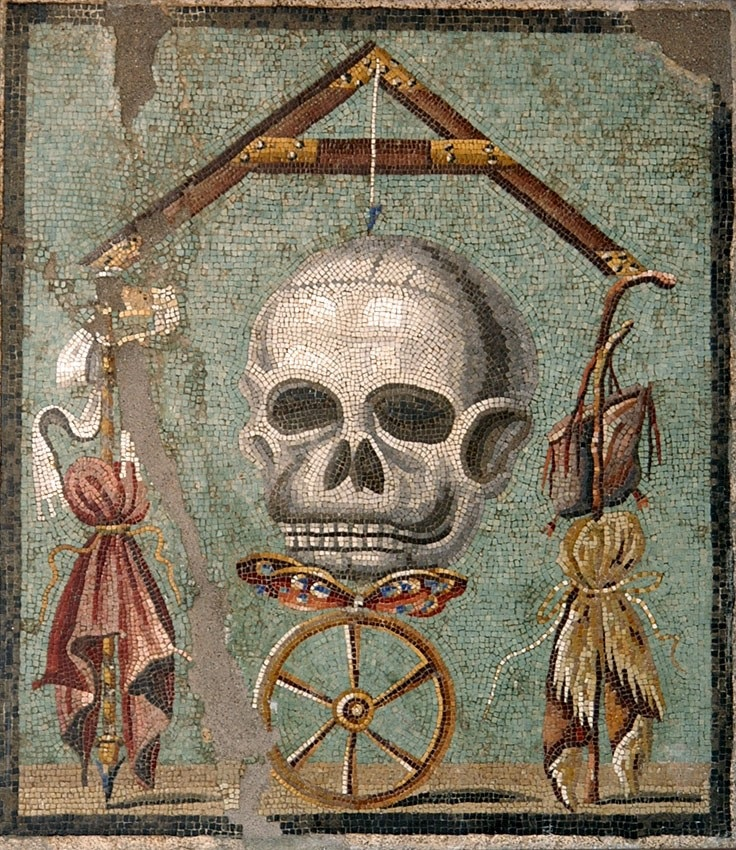
\includegraphics[width=\linewidth]{figures/Heekeren_fig1}
\caption{Memento Mori mosaic, in the Museo archeologico Nazionale di Napoli (Creative Commons License)}
\label{fig:heekeren_fig1}
\end{figure}
	The dining room or triclinium was named after the three rectangular couches, which were located around the sides of the room. Dinners were important in Roman social life. Dinners, as an event, were not only for the meeting of friends, but were also important for creating political alliances and as a display of status \parencite [119] {Ellis_1991}. According to \textcite [105-106] {Kondoleon_1991} it is possible to reconstruct the cultural context of mosaics based on their themes, arrangements, and their placements within the Roman house. This mosaic belongs to the so called emblemata, which were primary placed in triclinia, peristyles, and gardens. They were carefully positioned to attract the attention of guests as centrepieces \parencite [97] {Stewart_2004}.

	The domestic display of widely known cultural motifs was a privilege and a duty. The message of this decoration depended on the realistic portrayal of these events, and at times, revealed facets of Roman social matters. The compositions of mosaics became codified in time. Artists had to rely on their vision for the execution of the artwork, but their perception and creation could have been influenced by what they witnessed, such as funerals executed as spectacles or festivals. Especially funerals of a grand scale, which often contained an element of entertainment, where the audience was not only present to show their last respects, but also to be impressed and inspired  \parencites[112]{Kondoleon_1991}[89]{Hope_2009}. The Roman calendar contained several festivals dedicated to the cult of the dead. An example is the Parentalia, a festival that took place in February and was dedicated to the commemoration of the ancestors. Other festivals are the Rosalia and Lemuria \parencite[123--124]{Erasmo_2012}. The cult of the dead was part of Roman life.	\textcite {Panofsky_1939} mentions that, although there are different levels in his method, they become entangled, allowing the analyst to interpret the object as a whole. To make a clear visual analysis the object has been divided in four segments: the first segment, dominated by the  head of the triangle; the second segments, the area dominated by the forms supporting the triangle on either side ; the third segment, the central area dominated by the skull; and the fourth segment, the area under the skull. The first and second level of these segments is discussed in the next section. In Section 4.2 the final interpretation, or as is mentioned by Panofsky as intrinsic meaning, of all the segments will be given. The different figures of the mosaic are portrayed on a background with several shades of blue and surrounded with a black line. At the bottom there are yellowish shadows visible. The artist of the mosaic creates depth by the use of colours. 
	
%	\subsection {Visual Analysis: First and Second Level}
	The\marginnote{Visual Analysis: First and Second Level} first segment is visible at the top where a triangle is made out of two beams with a supporting beam in-between, with metal cappings and bolts visible. This triangle is supported on the right and left side. There is a line hanging from the middle of the triangle. This triangle represents a libella, which is a craftsman’s tool. This is one of the oldest technical measuring instruments, and known to be used by the Egyptians. The carpenter’s square, is a present version of this tool. When the libella was used in combination with a plumb line the craftsman was able to draw straight lines and perpendiculars \parencite [84] {Cuomo_2007}. Instead of hanging a piece of lead from the plumb line, there is a skull hanging from the carpenter’s square. 

	The second segment contains two elements, one on the left and one to the right, each supporting the triangle. The left side of the mosaic is damaged, but much of it is still visible. The left part, supporting the triangle, is a pole with diagonal stripes. Extra decoration is visible around this pole. At the top it looks like a white ribbon and at the bottom a reddish purple, most likely purpura, fabric are tied together with a strap or rope. On the right side, where the triangle is also supported, it looks like a wooden branch rather than a pole. It is decorated with something brown hanging from the branch, this might represent a bag. There is also yellow fabric hanging from the branch, and it looks damaged or torn. It seems that both these fabrics are tied together like dresses.
	The purpura fabric is draped in the shape of a dress around a sceptre. The damaged part of the mosaic with the white ribbon is interpreted by scholars as a crown. The purpure dress, sceptre, and crown together represent the rich and noble people. On the right side the libella is supported by a stick, travelling cloak and satchel. This side represents the poor people. Both sides represent the worldly goods which are taken away by death \parencites[99--100]{Cuomo_2007}[9]{Sogliano_1874}. 

	The third segment is visible in the centre of the mosaic. The line from the triangle is connected with this round, white with black object which is a skull. This skull is not true to nature in representing a human skull, and is possibly crafted after the skull of a monkey or other cranially-similar animal. However, the whole composition of the mosaic deals with a human aspect, so it is most likely that the skull represents a human skull and visualises death \parencite [99] {Cuomo_2007}. The afterlife was important in the Roman worldview. The disposal of the body had to be done in the right way following strict rituals, otherwise the soul of the departed would not achieve rest. Cremation became the dominant rite in the first century BC until the second century AD. A reason for this trend, as suggested by ancient commentators, is that people feared that non-cremated bodies might be exhumed or abused \parencite [80--82] {Hope_2009}. This mosaic was made mid-first century BC, so therefore, it was unlikely that the skull depiction was modelled after a real human skull, as there were no human skull available due to cremation trends at this time.
	
	The fourth segment, at the bottom of the mosaic, depicts two figures. There is a round object, which could represent a wheel. On top of this object there are two brightly ellipse forms with a white connection. This could be the representation of a butterfly or a dragonfly. However, it is more likely that this is a depiction of a wheel and a butterfly. In the Roman world the butterfly was a representation for the sensitive soul who left the earth \parencite [9] {Sogliano_1874}. The wheel means the wheel of fortune\parencite [99] {Cuomo_2007}.
	
%\subsection {Visual Analysis: Third Level and Final Interpretation}
This\marginnote{Visual Analysis: Third Level and Final Interpretation} mosaic is part of the Roman worldview on death. The Carpe Diem or ‘Seize the Day’ theme took a central place in the Roman society. Death and feasting were closely connected to the rite of passage. This association is visible in the ‘Memento Mori’ mosaic and the context in which it was found. However, there are also other examples, for instance the silver cups with dancing skeletons from Villa Boscoreale. Another example, from Pompeii, is a black and white mosaic from the House of the Faun, which depicts a skeleton carrying wine jugs, dated to the first century \AD This type of imagery should not be seen in a sombre or serious way.  The depictions carry a certain playfulness, in which the imagery suggests an acceptance of death \parencite [25--27, 85--87]  {Hope_2009}. It may also be the case that these objects were not used in a ritual manner. Rather it can be seen as a hymn to life, and the incorporation of death in daily life. Even though death and feasting have a strong connection, it does not mean the ‘Memento Mori’ must have served a funerary purpose. 

	\textcite{Hope_2009} also mentions that the afterlife for the Romans was important; although, there was not a consensus about what it looked like, how to reach it, and what was exactly important about it. This makes the ‘Memento Mori’ mosaic an opinion on death, and what was important for the afterlife.
	The piece shows the rich and the poor are equal in death. At this point social status was no longer important. It appears that one’s soul and fortune are the most important, because they are connected with the skull and hanging from the plumb line. It might even be possible that one’s soul and luck balance out what kind of afterlife one can receive.
	The Roman worldview on death can also be seen in a larger context: the cult of the dead. Drinking and eating was part of the rituals around funerals. There were food offerings for the dead, but also banquets after funerals to honour the dead and celebrate life \parencite [121--123] {Erasmo_2012}. Although these rituals were important to the Romans, it does not seem that there was a connection between this mosaic and funerary rituals because of the context in which it was found. The eat-and-drink theme was a common imagery at funerary monuments in the first century \AD, but these were almost never depicted with decaying bodies or skeletons. The image of the deceased shows them alive, non-skeletal and sometimes reclining as if at a feast \parencite[38]{Hope_2009}.

The imagery of the ‘Memento Mori’ mosaic is not unique, as mentioned by \textcite[99--100] {Cuomo_2007}. 
In the area of Campania a bronze weight from a steelyard was found dating from the same period as the mosaic. This weight is in the shape of a skull with a butterfly on top. Because there are more objects with the same visual depictions it is more likely that this combination of features had a special role in Roman society and their worldview at this time. This is also supported by \textcite{Perry_2005}  who argues that decorum explains the repeated use of certain visual concepts in Roman art. 
	
%	\section {Discussion and Conclusion}
The\marginnote{Discussion and Conclusion} context of the ‘Memento Mori’ mosaic is well known as it was a table adornment in a triclinium in a house in Pompeii. It was dated by the Museo archeologico Nazionale di Napoli to between 40 \AD and 60 \AD This case study shows that it is possible to use the three-levelled approach of \textcite{Panofsky_1939}  in an iconographic analysis of a Roman archaeological object. The ‘Memento Mori’ is a small piece, but it contains elements with intrinsic meaning. The mosaic is a vision on death; the rich and the poor are equal, the soul is leaving the ‘sphere of life’, and the wheel represents fate. A likely scenario is that it served as a part of the Carpe Diem worldview as suggested by \textcite {Hope_2009}. To come to this content it is useful to follow the levels offered by Panofsky. In the case of a simpler piece, it might not be necessary to use this method. Panofsky’s approach can assist in the analysis of more complex object pieces; but because of the exclusion of the context, it cannot give all the answers for archaeologists. However, this method can give guidance within analysis, to overcome the bias between nth{21} century thinking and that of the time the object is produced. This approach can connect the structure (worldview) of an ancient society to an expression of that worldview in the form of an object. The interaction between the object and viewer might be reached by following the levels, in order to come to meaning.

	Why the mosaic was placed on a dining table remains unclear. The visual meaning of the mosaic is explainable through Panofsky’s method, but it does reveal anything about why it was placed in this particular context. This problem was already suggested in section three and in this case study the iconography cannot explain the context. Do we actually know that it was used as a dining table or is it just an assumption based on what others have already interpreted? The meaning of an object in its context is equally important to iconographical detail, because context can change the meaning. Perhaps, the answer can be found in a combination of an object-centred approach to agency and how it affects human actions as argued by \textcite [196--197] {Gosden_2005}. Gosden mentions that the crucial context for an object, is the presence of other objects of the same style. Maybe a future study with comparable objects, for instance, the silver cups from Villa Boscoreale, can give an answer on the combination of context and meaning of an object.
	It is important to explore archaeological objects through iconographical analysis, as they can give new insights into ancient societies’ worldviews. Iconographical analysis is often strongly influenced by the social and cultural background of the executor, which creates an extra bias. Through this three-levelled method, objects can be interpreted in an impartial way. It has to be taken into account that an object is the opinion of a craftsman or a client and it does not have to represent a general idea. 
	Archaeologists work with objects in context, and the combination of this context and the interpretation of the visual culture are paramount for a better understanding. Panofsky’s method can be used well for the iconographical analysis of an object, but cannot tell archaeologists anything about context. Therefore, a misleading interpretation could be made, if only Panofsky’s method is used for the analysis of archaeological objects. A multidisciplinary approach, combining Panofsky’s approach with the contextual information derived from archaeological analysis will greatly benefit the analysis of archaeological objects.
	\myseparator
%	\section {Acknowledgment}
	I\marginnote{Acknowledgment} thank Dr. A. Rojas Martinez Gracida and Dr. E.M. Mol for their encouragement and support.
	
	\begin{myabstract}
		\foreignlanguage{italian}{%
			L'arte\marginnote{Abstract (Italian)} e gli oggetti romani sono stati fonte di produttiva discussione tra gli accademici, e questo ha portato allo sviluppo di successive teorie in merito. La ricerca tradizionale è stata influenzata, per esempio, da Winckelmann e dalla Kopienkritik. Queste teorie sono state utili nel comprendere l'arte romana, mancando però di un approccio oggettivo. Nel 1939 Erwin Panofsky ha pubblicato il volume Studies in Iconology introducendo un approccio a tre livelli per l'analisi delle strutture iconografiche dell'arte Rinascimentale. Questo articolo esamina l'applicazione dell'approccio a tre livelli di Panofsky al mosaico romano Memento-Mori al fine di evidenziare se esiste una sua utilità nel comprendere le evidenze archeologiche. Lo scopo è quello di sviluppare una analisi visuale, multidisciplinare, contestualizzata dell'oggetto in esame utilizzando tecniche pertinenti e all'ambito archeologico e all'ambito della storia dell'arte, al fine di evidenziare la sua compatibilità per l'interpretazione della cultura materiale del passato.}
	\end{myabstract}
		

\printbibliography[heading=subbibnumbered] 
\label{heekeren:lastpage}
\closingarticle